\documentclass{beamer}
\XeTeXlinebreaklocale "zh"
\XeTeXlinebreakskip = 0pt plus 1pt

\usetheme{CambridgeUS}
\usepackage[most]{tcolorbox} 
\usepackage{fontspec}
\usepackage{tikz}
\usepackage{amsmath, amssymb}
\usepackage{hyperref}
\setmainfont{Noto Serif CJK TC}
\setsansfont{Noto Sans CJK TC}
\setbeamertemplate{background}{
    \tikz[overlay, remember picture]\node [opacity=0.2] at(current page.east)[below=2cm, left = 0.2cm]{
\includegraphics[width=4cm]{logo.png}};
}

\AtBeginSection[]
{
 \begin{frame}<beamer>
 \frametitle{Outline}
 \tableofcontents[currentsection]
 \end{frame}
}
\AtEndDocument{\begin{frame}
\centering \Huge
                  Q \& A
               \end{frame}
                }
\title{Preliminaries of Cloud Security}
\author{Jianan Hong, \href{mailto:hongjn@sjtu.edu.cn}{hongjn@sjtu.edu.cn}}

\begin{document}
\begin{frame}
\titlepage
\end{frame}

\frame{\frametitle{Outline}
\tableofcontents%[pausesections]
}
\section{双线性配对}

\frame{\frametitle{Bilinear Pairing}
A mapping $e$ works on three order-$q$ groups ($\mathbb{G}_1, \mathbb{G}_2, \mathbb{G}_T$) as $$e: \mathbb{G}_1\times \mathbb{G}_2 \rightarrow \mathbb{G}_T$$

\begin{tcolorbox}[enhanced,colframe=white,colback=white, fuzzy halo = 1.3mm with gray]
\begin{enumerate}
\item \textcolor{red}{Bilinearity}. $\forall a, b \in \mathbb{Z}_p^2$, $u, v\in \mathbb{G}_1\times \mathbb{G}_2$: $e(u^a, v^b) = e(u,v)^{ab}$
\item \textcolor{red}{Non-degracy}. $u$ and $v$ are generators of $\mathbb{G}_1$ and $\mathbb{G}_2$: $e(u,v)$ generates $\mathbb{G}_T$.\footnote{$e(u,v)$的所有幂次取遍群里的所有元素}
\item \textcolor{red}{Efficiency}. $e$ is a polynomial-time algorithm for all $u,v$.
\end{enumerate}
\end{tcolorbox}
}
\frame{
	\frametitle{配对中的必要解释}
	在密码算法设计中,一般不需要了解具体用了什么数学工具实现了这种操作。

	\begin{itemize}
		\item 一般来说, $\mathbb{G}_T$是乘法群,但$\mathbb{G}_1, \mathbb{G}_2$有被写成加法群,也有被写成乘法群。
		\item 当写成加法群时,双线性特性写成 $e(aP, bQ) = e(P,Q)^{ab}$
		\item 因为群只有一种运算,写法对方案影响不大
	\end{itemize}
	从安全上看,凡是无法从群元素运算,以及配对运算计算的结果都可认为是无法运算的。在密码学上,也特别定义了一些难题,典型的比如BDH
\begin{tcolorbox}[enhanced,colframe=white,colback=white, fuzzy halo = 1.3mm with gray]
	A BDH tuple is as $(g_1, g_2, g_1^a, g_1^b, g_2^c, e(g_1,g_2)^{abc})$
	\begin{itemize}
		\item BDH tuple is difficult to determine or compute.
	\end{itemize}
\end{tcolorbox}
}
\frame{
	\frametitle{BLS signature: 从CBDH难题产生的签名算法}
	\begin{itemize}
		\item \alert{SK} $SK = x \in \mathbb{Z}_q$
		\item \alert{PK} $PK = g_1^x$
		\item \alert{Sign} $\sigma = H(m)^x$
		\item \alert{Verify} check if $e(g_1, \sigma)= e(PK, H(m))$
	\end{itemize}

\vskip 0.2cm

\alert{NOTE:} 某些配对曲线中,$\mathbb{G}_1$和$\mathbb{G}_2$一致,直接写作$\mathbb{G}$
}
\section{线性秘密共享LSSS}
\frame{\frametitle{Lagrange Interpolation}
Any degree-$t-1$ polynomial $$P(x) = \sum_{i=0}^{t-1} a_i x^i$$
can be reconstructed from $t$ distinct points in the curve \footnote{Instance: a degree-2 curve is determined by 3 points}. 

\begin{tcolorbox}[enhanced,colframe=white,colback=white, fuzzy halo = 1.3mm with gray]
With $t$ points $(x_i, y_i = P(x_i))$
$$P(x) = \sum_{1\leq i\leq t} l_i y_i$$
$$ l_i = \prod_{1\leq j\leq t}^{j\neq i} \frac{x - x_j}{x_i - x_j} $$
\end{tcolorbox}
}
\frame{\frametitle{理解每一项的物理含义}
\begin{itemize}
	\item 首先确认唯一性。在此前提下,任何方法构造出来的多项式都是确定性的。
\end{itemize}

\begin{tcolorbox}[enhanced,colframe=white,colback=white, fuzzy halo = 1.3mm with gray]
	\begin{itemize}
		\item 构造了t个多项式$P_i=w_i\prod_{1\leq j\leq t}^{j\neq i}(x-x_j)$
			\begin{itemize}
				\item $P_i$ 是在除$x_i$外,其他指定点取之为0的多项式;
				\item 那么,对任意$F(x)$,$P_i+F(x)$在其他给定点$x_j\neq x_i$的值$$F(x_j)+P_i(x_j) = F(x_j)$$
			\end{itemize}
		\item 只需调整$w_i$,使$P_i(x_i) = y_i$
			\begin{itemize}
				\item $w_i = y_i /\prod_j (x-x_j)$
			\end{itemize}
		\item $P(x) = \sum P_i$
	\end{itemize}
\end{tcolorbox}
}
\frame{\frametitle{LSSS 的另一种表示方法}
高维空间上选择一个点
\begin{enumerate}
	\item 在$n$维空间中有互不平行的超平面
	\item $n$个超平面相交于一个点
\end{enumerate}

\vskip 1cm

To express a hyperplane in an \alert{n-dimension} span:
\begin{itemize}
	\item a n-dimension vector: $$(e_1, e_2, \dots, e_n)\cdot \vec{x} = c$$
	\item 互不平行的超平面:线性无关向量
\end{itemize}
}

\frame{
	\frametitle{Hyperplane: Continue}
	考虑$n$个线性无关向量穿过一个点$\Omega \in \mathbb{R}^n$
$$(s_1, s_2, \dots, s_n) \gets 
\begin{pmatrix}
	e_{1,1} &  \cdots & e_{1,n} \\
	\vdots & \ddots & \vdots \\
	e_{n,1} & \cdots & e_{n,n}
\end{pmatrix}
\cdot \Omega
$$
\begin{itemize}
	\item $s_i$ 就是隐藏$\Omega$的秘密信息
	\item 如果想从$s_i$恢复$\Omega$,只需要找到逆矩阵
\end{itemize}
}
\frame{
	\frametitle{LSSS的效果}
	\begin{itemize}
		\item \alert{高效性} 只要凑够足够的share,得到秘密的算法是高效的;
		\item \alert{秘密性} 只要没有凑够,那么对秘密的知识量为0
			\begin{itemize}
				\item 对于多项式。确定其他$t-1$个点,修改第$t$个点,秘密值取遍空间;
				\item 对于超平面,确定其他平面,另一个平面的值能让秘密值取遍全空间。
			\end{itemize}
		\item 一般来说,秘密值是多项式的$P(0)$或空间中点的第一维数值。
	\end{itemize}
}
\section{Paillier Cryptosystem}

\frame{\frametitle{Algorithm}
Big primes $p, q$ are securely chosen:
\begin{enumerate}
	\item $n=pq, \lambda = lcm(p-1, q-1)$, select $g\in \mathbb{Z}_{n^2}^*$. 可以为2
	\item $\mu = (L(g^\lambda \mod n^2))^{-1} \mod n$. \alert{L(x) = (x-1)/n}
	\item pk = $n,g$. sk = $\lambda, \mu$
\end{enumerate}

先不考虑私钥格式与解密,先看加密方法:
\begin{enumerate}
	\item 明文$0\leq m\leq n$;
	\item 选择 $r$ 与 $n$ 互质;
	\item 密文 $c = g^m \cdot r^n \mod n^2$
\end{enumerate}
}

\frame[label={crs}]{\frametitle{具体算法:可信第三方根据限制t和最大多项式次数d构造参数crs}
\begin{enumerate}
\item \hyperlink{noname}{select random $s, \alpha$}
\begin{itemize}
\item $s$ is a point to evaluate polynomial; 
\item $\alpha$ is shift to restrict polynomial.
\end{itemize}
\item get $g^\alpha$, $\{g^{s^i}\}_{1\leq i\leq d}$, $\{g^{\alpha s^i}\}_{1\leq i\leq d}$
\item for prover: crs is 
$$ \{g^{s^i}\}_{1\leq i\leq d}, ~ \{g^{\alpha s^i}\}_{0\leq i\leq d} $$
\item for verifier: vrs is 
$$ g^\alpha, g^{t(s)}$$
\end{enumerate}
}

\frame{\frametitle{Prove:}
Input:
\begin{tcolorbox}[enhanced,colframe=white,colback=white, fuzzy halo = 1.3mm with gray]
\begin{itemize}
\item crs = $ \{g^{s^i}\}_{1\leq i\leq d}, ~ \{g^{\alpha s^i}\}_{0\leq i\leq d} $
\item polynomial $h(x), p(x)$
\end{itemize}
\end{tcolorbox}

\begin{enumerate}
\item evaluate $g^{p(s)}, g^{h(s)}$. \footnote{e.g., let $p(x) = \sum a_i x^i$, then $g^{p(s)} = \prod (g^{s^i})^{a_i}$, especially, $g^{s^i}$ is in crs}
\item evaluate $g^{\alpha p(s)}$
\item proof output $\pi = (g^{ p(s)}, g^{ h(s)}, g^{ \alpha p(s)})$
\end{enumerate}

\alert{It is easy to verify that in $\pi = (A, B, C)$}
$$ e(A, g) = e(g^{t(s)}, B)$$
}

\frame[label={polynomial}]{\frametitle{Verify:}
Input:
\begin{tcolorbox}[enhanced,colframe=white,colback=white, fuzzy halo = 1.3mm with gray]
\begin{itemize}
\item 证明信息 = $ \pi = (A, B, C) = (g^{ p(s)}, g^{ h(s)}, g^{ \alpha p(s)}) $
\item crs =  $g^\alpha, g^{t(s)}$
\end{itemize}
\end{tcolorbox}

\begin{enumerate}
\item 验证多项式满足整除限制 $p(s) = t(s)\cdot h(s)$
$$e(A, g) = e(g^{t(s)}, B)$$
\item 验证多项式$p(X)$存在的真实性
$$e(A, g^\alpha) = e(C, g)$$
\end{enumerate}
}

\frame{\frametitle{多项式证明总结}
如果一个问题可分解为某个多项式$p(X)$被具有特殊意义的多项式$t(X)$整除。则\alert{该问题可被snark高效证明}。

\vskip 1cm
\begin{tcolorbox}[enhanced,colframe=white,colback=white, fuzzy halo = 1.3mm with gray]
进一步说明
\begin{itemize}
\item 比如,要声明$p(X)$ 在点$(x_1, x_2, \dots, x_k)$取值为0。
\item 则$t(X) = \prod (X-x_i)$.
\end{itemize}
另一方面
\begin{itemize}
\item 在结合实际电路证明问题时,验证者也掌握$p(X)$的部分信息。
\item 如,电路的部分公开信号statement
\item 因此,除本节所提到的证明外,还需要额外证明$A=g^{p(s)}$满足statement限制。
\end{itemize}
\end{tcolorbox}
}
\section{从QAP到多项式,如何构造$p(X)$}
\frame{\frametitle{电路的high-level视角看必要标识}
	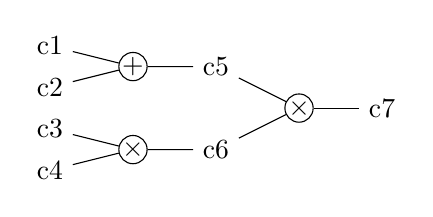
\begin{tikzpicture}[grow=left,
	level 2/.style={sibling distance=3em},
	level 4/.style={sibling distance=1.5em}, level distance=3em]
		\node {c7}
		child { node [draw, circle, inner sep=0mm]{$\times$}
		child {node {c5}
		child {node [draw, circle, inner sep=0mm]{$+$}
		child {node {c1}}
		child {node {c2}}
		}}
		child {node {c6}
		child {node [draw, circle, inner sep=0mm]{$\times$}
		child {node {c3}}
		child {node {c4}}
		}}
		};
	\end{tikzpicture}
\begin{itemize}
	\item 整个QAP电路包含多个信号$c_i$和多个算符
	\item 算符包含乘法和加法,其中加法可被高效方法等效省略
	\item 信号包含输入,输出,和中间值。
	\item 每个算符包含2个输入(left, right)和1个输出。
\end{itemize}
}

\frame{\frametitle{第$i$个算符}
\begin{tcolorbox}[enhanced,colframe=white,colback=white, fuzzy halo = 1.3mm with gray]
\centering
	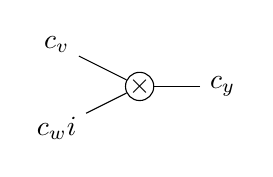
\begin{tikzpicture}[grow=left,
	level 2/.style={sibling distance=3em},
	level 4/.style={sibling distance=1.5em}, level distance=3em]
		\node {$c_y$}
		child { node [draw, circle, inner sep=0mm]{$\times$}
		child { node {$c_v$}}
		child { node {$c_wi$}}
		};
	\end{tikzpicture}
	$v_i, w_i, y_i$分别为算符的左右输入键和输出键。
\end{tcolorbox}
思维逻辑:
\begin{itemize}
\item 信号限制:$c_v \times c_w - c_y = 0$
\item 使$u,w,v$为三个多项式,为算符赋值unique index $r_i$:
	\begin{itemize}
	\item Let $v_i(r_i) = w_i(r_i) = y_i(r_i) = 1$
	\item Let $v_i(r_j) = w_i(r_j) = y_i(r_j) = 0$ for $j\neq i$
	\item 扩展信号限制 $c_vv_i(r_i) \times c_ww_i(r_i) - c_yy_i(r_i) = 0$
	\end{itemize}
\end{itemize}
}

\frame{\frametitle{令所有信号限制得到满足}
遍历所有信号$c_1$ 到 $c_m$,有
$$(\sum_{k=1}^m c_k v_k(r_i)) \cdot (\sum_{k=1}^m c_k w_k(r_i)) - (\sum_{k=1}^m c_k y_k(r_i)) = 0$$
\begin{tcolorbox}[enhanced,colframe=white,colback=white, fuzzy halo = 1.3mm with gray]
解析:
\begin{itemize}
\item 对于某个算符$i$,它的相关信号的系数$$v_i(r_i) = w_i(r_i) = y_i(r_i) = 1$$
\item 无关信号的系数为0。
\item 因此,对任何电路内的算符,sum中仅剩下相关输入/输出的信号$c_k$
\end{itemize}
\alert{则,所有算符都可解析为$c_v \cdot c_w - c_y = 0$}
\end{tcolorbox}
}

\frame{\frametitle{构造多项式}
令上一页公式为多项式$p(X):$
$$p(X) = (\sum_{k=1}^m c_k v_k(X)) \cdot (\sum_{k=1}^m c_k w_k(X)) - (\sum_{k=1}^m c_k y_k(X))$$
\vskip 0.4cm

\begin{itemize}
   \item Let $\sum c_k v_k(X) = v(X)$, so as $w(X)$ and $y(X)$
   \item Generate $v, w, y$ with Lagrange Interpolation.
   \item \alert{每个多项式都由算符赋值点$r_i$函数值限制}
\end{itemize}

由于$v, w, y$的最高次数都是电路乘法算符个数-1,因此$p(X)$的次数2倍于算符个数。
}

\frame{\frametitle{构造限制多项式t(X)}
构造t(X),该多项式在每个算符赋值点的函数值为0。
$$t(X) = \prod (X-r_i)$$
}

\frame[label={QAP}]{\frametitle{多项式的构造特点}
\begin{itemize}
   \item $t(X)$ 只和电路形式相关,和具体信号无关。进一步,之和电路内乘法算符相关。
   \begin{itemize}
   \item $t(X)$ 因此$t(X)$可被任何人构造,无需知道对应秘密。
   \end{itemize}
   \item $p(X)$ 与信号值相关,只有拥有完整电路信息的实体可以构造
   \item $h(x) = p(X)/t(X)$ 必须通过$p(X)$,也必须掌握全套信息。
\end{itemize}

\begin{tcolorbox}[enhanced,colframe=white,colback=white, fuzzy halo = 1.3mm with gray]
结合\hyperlink{set}{多项式的零知识证明}方法,prover已经拥有向别人证明自己拥有任何问题求解的能力
\end{tcolorbox}
}

\section{What Remains: public statement}

\frame{\frametitle{Additionally prove statement in P(X)}
Revisit $v(X)$ as $$v(X) = \sum_{k=1}^m c_k v_k(X)$$

\alert{Note: Let $v_k(X)$ be a polynomial} be like 
\begin{align}
v_k(x) = \begin{cases}
1 & x=\text{the gate}\\
0 & x=\text{other gate}
\end{cases} 
\end{align}
$v_k(x)$ can be interpolated by any party. As so as $w_k, y_k$
}

\frame[label={noname}]{\frametitle{修改$v,w,y$的多项式构造方法 (use v as instance)}
$$v = \sum_{k=1}^m c_k \cdot (v_k(X))$$
Small difference is $v_k(X)$ is already a polynomial generated in public.
\vskip 0.3cm

\line(1,0){450}

%\begin{tcolorbox}[enhanced,colframe=white,colback=white, fuzzy halo = 1.3mm with gray]
In such way, by chosing index $s$ \hyperlink{crs}{to evaluate polynomial}:
\begin{enumerate}
\item TPS evaluate $v_k(s)$ directly as an integer.
\item Prover can evaluate $c_kv_k(s)$ without knowing $s$ for every signal.
\item Verifier can evaluate $c_kv_k(s)$ for every statement.
\end{enumerate}

%\end{tcolorbox}
}

\frame{\frametitle{微调多项式证明方法}
本页忽略关于shift的使用
\line(1,0){450}

\begin{columns}
\column{0.4\textwidth}
Let $g\in\mathbb{G}_1, h\in\mathbb{G}_2$
\begin{tcolorbox}[enhanced,colframe=white,colback=white, fuzzy halo = 1.3mm with gray]
In crs, provides:
\begin{footnotesize}
\begin{itemize}
\item $\{g^{v_k(s)}, h^{w_k(s)}, g^{y_k(s)}\}$
\item $g^{s^i}, i\leq d$
\item $h^{t(s)}$
\end{itemize}
\end{footnotesize}
\end{tcolorbox}
\column{0.6\textwidth}
\begin{enumerate}
\item Prover provides 
\begin{align}
A = &\prod (g^{v_k(s)})^{c_k}\\
B =& \prod (h^{w_k(s)})^{c_k}\\
C = & \prod (g^{y_k(s)})^{c_k}\\
H = & g^{h(s)}
\end{align}
\item $e(A,B)/e(C, h) =e(g^{p(S)}, h) = T$
\item $T = e(H, h^{t_s})$
\end{enumerate}
\end{columns}
}

\frame{\frametitle{Add Statement in Snark}
\begin{enumerate}
\item In proof, the A, B, C are summed with only witnesses.
\item The verifier supplies ultimate A, B, C with proof.
\end{enumerate}
}

\frame{\frametitle{Overall.Gen}
Let public statement be $c_1$ to $c_N$ and witness $I_m$ be $c_{N+1}$ to $c_m$
\begin{itemize}
\item Select random $s, \alpha,\beta_v, \beta_w, \beta_y$
\item crs is 
\end{itemize}

\begin{align}
\{g^{s^i}, g^{\alpha s^i}\}_{i=0}^d\\
h^{\beta_v}, \{g^{\beta_v v_i(s)}\}_{i\in I_m}\\
h^{\beta_w}, \{g^{\beta_w w_i(s)}\}_{i\in [m]}\\
h^{\beta_y}, \{g^{\beta_y y_i(s)}\}_{i\in [m]}
\end{align}
}

\frame{\frametitle{Overall.Prove}
\begin{itemize}
\item $v_m = \sum_{i\in I_m} c_i v_i(x)$
\item $H = g^{h(s)}, \hat{H} = g^{\alpha h(s)}$
\item $V_m = g^{v_m(s)}, \hat{V_m} = g^{\alpha v_m(s)}$
\item $W = h^{w(s)}, \hat{W} = h^{\alpha w(s)}$
\item $Y = g^{y(s)}, \hat{Y} = g^{\alpha y(s)}$
\item $B = g^{\beta_vv(s)+\beta_ww(s)+\beta_yy(s)}$
\item proof is $\pi = (H,\hat{H}, V_m, \hat{V_m}, W, \hat{W}, Y, \hat{Y}, B)$
\end{itemize}

Note that $h$ and $h(x)$ means different.
}

\frame{\frametitle{Overall.Verify}
\begin{itemize}
\item Shift Verify. $e(H, h^\alpha) = e(\hat{H}, h)$, so as $V_m, W, Y$
\item Complete V as $V = V_m \cdot \prod_{i\in [N]}g^{c_i v_i(s)}$
\item Check polynomial restriction. $e(H, h^{t(s)}) = e(V, W)/e(Y,h)$
\item Check Linear span. $e(B, h) = e(V, h^{\beta_v})\cdot e(W, h^{\beta_w})\cdot e(Y, h^{\beta_y})$
\end{itemize}
}
\frame{
	\frametitle{Snark Analysis}
	It is not zero knowledge: to realize \alert{Zk-SNARK} from \alert{SNARK}, additional blindness is required.
\begin{tcolorbox}[enhanced,colframe=white,colback=white, fuzzy halo = 1.3mm with gray]
	\begin{itemize}
		\item ZKP can be proved if every element is distributed identical to random chosen.
		\item try W as instance: a modification as $W = h^{w(s)+\delta}$ instead of $h^{w(s)}$
		\item the prover provides remainder $e(V,h^{\delta})$ to make verification pass.
	\end{itemize}
\end{tcolorbox}
\vskip 0.8cm

In fact, there is a more efficient scheme realizing zk-snark, even faster than the presented SNARK. Refer to [Gro16] Jen Groth. ``On the Size of Pairing-based Non-interactive Argument.'' 2016.
}
\end{document}
